%Autonomous driving in urban environments: Boss and the urban challenge,
%Visual odometry and mapping for autonomous flight using an rgb-d camera
%  “The planner ensemble and trajectory executive: A high performance motion planning system with guaranteed safety
%Y. Zhu, R. Mottaghi, E. Kolve, J. J. Lim, A. Gupta,L. Fei-Fei, and A. Farhadi. Target-driven visual navigation in indoor scenes using deep reinforcement learning. In Proc. ICRA, 2017.
%C. R. Qi, W. Liu, C. Wu, H. Su, and L. J. Guibas. Frustum pointnets for 3d object detection from rgb-d data. arXiv:1711.08488, 2017
%R. B. Rusu, Z. C. Marton, N. Blodow, M. Dolha, and M. Beetz. Towards 3D Point Cloud Based Object Maps for Household Environments. Robotics and Autonomous Syst
% A. Golovinskiy, V. G. Kim, and T. Funkhouser. Shapebased recognition of 3d point clouds in urban environments. In Proc. ICCV, 2009.


%Mamic, G. and Bennamoun, M. (2002). Representation and recognition of 3D free-form objects. Digital Signal Processing, 12(1):47–76. 3D object recognition has been extensively investigated during the last two decades due to the availability of low cost scanners and high speed computing devices
\chapter{Tổng quan}
\label{chap-intro}
\begin{ChapAbstract}
Trong chương này, nhóm sinh viên giới thiệu ngắn gọn nội dung của đề tài khóa luận, sự quan trọng của thông tin ba chiều trong cuộc sống thông qua các ứng dụng, đặc biệt là ứng dụng liên quan tới nhận dạng và truy vấn vật thể ba chiều, các kĩ thuật thu thập dữ liệu ba chiều và các loại cảm biến. Sau đó, nhóm sinh viên trình bày lý do thực hiện đề tài, mục tiêu đề tài và tổng quan của toàn bộ khóa luận.
\end{ChapAbstract}


\section{Giới thiệu chung}
Lĩnh vực thị giác máy tính là lĩnh vực tìm cách giải quyết vấn đề để máy tính nắm bắt được các thông tin và nội dung mức độ cao từ thông tin thị giác, ví dụ ảnh, video, độ sâu... Hiện nay, với sự phổ biến của những thiết bị thu thập dữ liệu, các cảm biến lĩnh vực thị giác máy tính được mở rộng để giải quyết các vấn đề trên kiểu dữ liệu ảnh ba chiều, ảnh y khoa. Đặc biệt, lĩnh vực ảnh ba chiều đang là một chủ đề được quan tâm nhiều hơn bởi sự xuất hiện của các thiết bị, cảm biến thu thập dữ liệu thông tin ba chiều và những nhu cầu thực tế yêu cầu máy tính hiểu và sử dụng được dữ liệu ba chiều. Sự phổ biến và giá thành phù hợp của các thiết bị, cảm biến thu thập thông tin ba chiều như các dòng camera Intel RealSense\cite{IntelRealSense}, Microsoft Kinect\cite{Kinect}, Matterport\cite{Matterport},v.v... làm cho dữ liệu ba chiều và những ứng dụng kèm theo trở nên phổ biến hơn. Ngoài ra, những năm gần đây, những ứng dụng có sử dụng đến thông tin ba chiều như thực tại tăng cường, thực tại ảo, xe tự lái, robot giao hàng, siêu thị tự động, chứng thực bằng khuôn mặt ba chiều,v.v... đã thúc đẩy những nghiên cứu về chủ đề thị giác máy tính trên dữ liệu ba chiều. Nội dung đề tài nhóm chúng em thực hiện nhằm tập trung nghiên cứu bài toán nhận dạng và truy vấn vật thể ba chiều. Cụ thể là nghiên cứu những phương pháp biểu diễn những dữ liệu ba chiều, những phương pháp truyền thống và những phương pháp áp dụng học sâu trên dữ liệu ba chiều. Vấn đề nhận dạng ba chiều được xem như nền tảng để tiếp tục nghiên cứu những vấn đề tiếp theo như phân đoạn vật thể trong không gian ba chiều, phát hiện vật thể trong không gian ba chiều, trong khi đó, vấn đề truy vấn dữ liệu ba chiều lại có tính áp dụng lớn và liên quan nhiều đến thực tiễn của nhu cầu tìm kiếm thông tin.


\subsection{Thông tin 3D}
Thị giác con người không chỉ có duy nhất nhận thức về màu sắc, thị giác con người còn có nhận thức về độ sâu, là khả năng nhận thức thế giới trong không gian ba chiều và khoảng cách tới một vật thể. Nhận thức về độ sâu có thể đến từ nhiều nguồn khác nhau, chẳng hạn kết hợp thông tin thị giác nhận được từ hai mắt (binocular), bao gồm các thông tin như độ sai lệch (disparity),... Nhận thức về độ sâu cung cấp cho con người những thông tin hữu ích, chẳng hạn định vị trong không gian, phỏng đoán khoảng cách xa gần và nhận diện vật thể, định vị vị trí vật thể trong tầm nhìn. Để mô phỏng đồ vật thực tế trên máy tính một cách chân thật, cũng như để máy móc có khả năng thực hiện một số công việc của con người, thông tin ba chiều của đồ vật là quan trọng. 

Ngoài ra, các vật thể ba chiều cũng được ứng dụng trong nhiều lĩnh vực, đồ họa máy tính, thị giác máy tính và rô bốt, thiết kế nhà cửa, công trình, thực tế ảo, mô phỏng các cấu trúc ba chiều phức tạp,... Trong đồ họa máy tính, chẳng hạn như làm trò chơi máy tính, vật thể ba chiều được sử dụng để tạo ra các môi trường ảo, nhằm tăng cường trải nghiệm người dùng trong thời gian chơi. Trong thị giác máy tính, thông tin 3D hữu ích trong các vấn đề, chẳng hạn dựa vào thông tin 3D có thể dự đoán một đối tượng là loại đối tượng nào trong trường hợp thiếu sáng, nhận diện khuôn mặt. Trong giáo dục, các vật thể ba chiều, các chuyển động ba chiều được giả lập để giúp học sinh hình dung rõ ràng hơn hiện tượng ngoài cuộc sống đời thực. Ngoài ra, thông tin 3D còn được sử dụng trong những lĩnh vực như thiết kế máy móc, hệ thống hoặc trang trí nội thất. Tóm lại, thông tin 3D đóng góp một phần rất quan trọng trong cuộc sống.

\subsection{Cảm biến độ sâu - 3D Sensor}
Để thu thập thông tin ba chiều, các cảm biến 3D đặc biệt được chế tạo. Cảm biến 3D là những cảm biến đặc biệt, có khả năng đo lường các thông tin như độ sâu, khoảng cách từ cảm biến tới vật thể, cấu trúc thông tin ba chiều của vật thể như hình dạng, độ cong, và có thể có khả năng  đo lường màu sắc... Dữ liệu sau khi thu thập được từ cảm biến 3D sau đó được tổng hợp lại và tạo thành các mô hình 3D. Có nhiều kĩ thuật khác nhau được sử dụng để tạo ra các camera ba chiều, tùy theo điểm mạnh, điểm yếu và giá thành, được chia làm hai kĩ thuật chính: kĩ thuật tiếp xúc (contact), không tiếp xúc (non-contact) \cite{3DSensorTypes}.

Các cảm biến 3D loại tiếp xúc đo lường vật thể bằng việc chạm trực tiếp vật lý trên vật thể, trong khi vật thể được đặt nằm yên không di dời trên một bề mặt bằng phẳng, vững chắc. Các cảm biến 3D loại tiếp xúc có khả năng tạo ra các mô hình 3D có độ chính xác cao so với vật thật và thường được dùng trong công việc chế tạo máy móc. Tuy nhiên, vì phải tiếp xúc trực tiếp với vật thể,  vật thể có thể bị hư hỏng sau khi bị tiếp xúc bởi các cảm biến 3D loại tiếp xúc. Ngoài ra, tốc độ thu thập thông tin của các cảm biến 3D loại này thường rất chậm.

Các cảm biến 3D loại không tiếp xúc đo lường vật thể dựa trên nguyên tắc chính là phát ra những tia sáng, hoặc bức xạ và phát hiện sự phản chiếu hoặc đi xuyên qua vật thể để đo lường thông tin của vật thể. Các loại tia này có khả năng là ánh sáng, sóng siêu âm hoặc x-ray. Một số kĩ thuật thường gặp là time-of-flight, đo lường khoảng thời gian từ lúc một tia được phát ra cho tới khi nhận lại để có được thông tin về vật thể, hoặc triangulation, sử dụng một camera khác để phát hiện vị trí phản xạ của một tia laser, từ đó rút ra được thông tin không gian của vật thể. Điểm mạnh của cảm biến camera loại không tiếp xúc là giá thành rẻ hơn và khả năng quét vật thể nhanh hơn. Tuy nhiên, độ chính xác của cảm biến loại này không cao do khó khăn trong việc tính toán thời gian di chuyển của ánh sáng (rất nhanh) trong kĩ thuật time-of-flight hoặc giới hạn phạm vi trong kĩ thuật triangulation.

\begin{figure}[H]
\centering
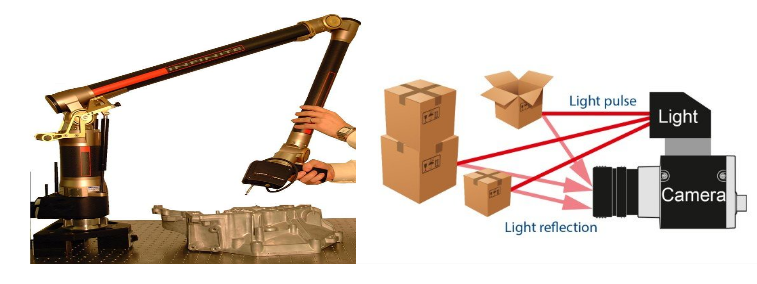
\includegraphics[width=\linewidth]{resources/chapter1_contact_noncontact3d.png}
\caption[Hai loại cảm biến 3D]{Hai loại cảm biến 3D. Cảm biến camera tiếp xúc (trái), và không tiếp xúc(phải)}
\label{fig:linear_nonlinear_data}
\end{figure}

